\documentclass[12pt]{article}

\usepackage[utf8]{inputenc}
\usepackage{subfig}
\usepackage{graphicx}
\usepackage{epstopdf}
\usepackage{amsmath}
\usepackage{fancyvrb}
\usepackage{fullpage}
\usepackage{paralist}

\title{Concurency and Multithreading\\
       Java concurrency Constructs}
\author{Alexandru Mosoi $<$ami650@few.vu.nl$>$\\
        student number 2000903}

\begin{document}
\maketitle


\section{Counter}

\begin{table}[h!]
  \centering
  \small
  \framebox{
    \begin{tabular}{ r | c | c | c | c | c }
    \# Threads & 1 & 2 & 3 & 4 & 8 \\
    \hline
    Simple & 2000000000 & 1000046618 & 670269482 & 500093260 & 252398649 \\
    Volatile & 2000000000 & 1370615635 & 1375495038 & 1414755523 & 1259676634 \\
    Synchronized & 2000000000 & 2000000000 & 2000000000 & 2000000000 & 2000000000 \\
    \end{tabular}
  }

  \caption{Counter value for variable N and K = 2.000.000.000 on a 4 logical
  cores processor}
  \label{tbl:counter}
\end{table}


Table \ref{tbl:counter} lists value of the counter after it was incremented
\texttt{K / N} times on \texttt{N} different threads, for a total of
\texttt{K} increments. The pseudo code executed by a thread is listed in
figure \ref{fig:counter-pseudocode}.

\begin{figure}[h!]
  \begin{Verbatim}[frame=single]
for (long i = 0; i < K / N; i++) {
  counter.inc();
}
  \end{Verbatim}
  \caption{Counter pseudocode}
  \label{fig:counter-pseudocode}
\end{figure}

\subsection{Simple}
\label{ssec:simple}

\emph{Simple} does not use any synchronization constructs. Java
HotSpot assumes that variable is not shared across multiple threads and
detects an optimization opportunity. The memory access into the following
pattern:

\begin{verbatim}
read counter into local-counter
increment local-counter K/N times
write local-counter to counter
\end{verbatim}

The last thread to execute \texttt{write local-counter} sets the final
value for shared counter. Since there are $N$ threads and each thread
increments the counter $K/N$ times the final value of the counter
will be at least $K/N$. The slight difference in the reported value
and the theoretical one is because of lazy runtime optimization of Java HotSpot.
Before the loop is optimized, the value might have been incremented separately
by all threads.

\subsection{Volatile}
\emph{Volatile} declares the internal counter as \texttt{volatile}.
This will disable optimizations and the memory access pattern changes to

\begin{verbatim}
repeat
  read counter into local-counter
  increment local-counter 1 time
  write local-counter to counter
\end{verbatim}

However when considering multiple threads, for example \texttt{t1} and
\texttt{t2}, the following \emph{race}\footnote{Both threads read the
same value, increment it and then write it back} is possible because
the incrementation is not atomic:

\begin{verbatim}
t1:read counter into local-counter

t2:read counter into local-counter
t2:increment local-counter 1 time
t2:write local-counter to counter

t1:increment local-counter 1 time
t1:write local-counter to counter
\end{verbatim}

Depending on the scheduling of the threads the final value of the counter can
take any value from 1 to \texttt{K}.

\subsection{Synchronized}

\emph{Synchronized} protects the access to internal counter with
the counter's monitor so no two threads will execute the critical
section simultaneously. The memory access pattern will be:

\begin{verbatim}
t1:in critical section
t1:  read counter into local-counter
t1:  increment local-counter 1 time
t1:  write local-counter to counter

t2:in critical section
t2:  read counter into local-counter
t2:  increment local-counter 1 time
t2:  write local-counter to counter
\end{verbatim}

The final value of the counter will always be equal to \emph{K}. This
implementation of the counter works as expected.


\newpage
\section{Search}

\begin{table}[h!]
  \centering
  \small
  \framebox{
    \begin{tabular}{ r | c | c | c | c }
    \# Threads & 1 & 2 & 3 & 4 \\
    \hline
    Simple & 50000001 & 75000001 & 83333333 & 87500001 \\
    Volatile & 50000001 & 45654166 & 56228251 & 68703196 \\
    \end{tabular}
  }

  \caption{Number of visited entries for variable N and K = 100.000.000 on a 4 logical
  cores processor. Reported values are averaged over 7 runs.}
  \label{tbl:search}
\end{table}

Table \ref{tbl:search} gives the average number of entries visited before the
value located at index $K / N / 2$ is found in a vector with $K$ elements
using $N$ threads. The value is always found by the first thread after
searching half of the elements assigned to it. The pseudo code executed by
a thread is listed in figure \ref{fig:search-pseudocode}. \texttt{found}
is a shared boolean variable set to \texttt{true} when the target value was
found by any of the threads.

\begin{figure}[h!]
  \begin{Verbatim}[frame=single]
for (i = start; i < end && !found; i++) {                                    
  if (table[i] == value) {                                                   
    found = true;                                                            
    break;                                                                   
  }                                                                          
}                                                                            
                                                                             
synchronized (Search.class) {                                                
  visited += visited_elements_in_current_thread;
}
  \end{Verbatim}
  \caption{Search pseudo code}
  \label{fig:search-pseudocode}
\end{figure}


\subsection{Simple}

\emph{Simple} doesn't use any synchronization mechanism. Similar to subsection
\ref{ssec:simple} Java HotSpot optimizes away reading of \texttt{found}
because it implicitly assumes that \texttt{found} flag is accessed by only
a thread and it changes only at the end of the loop. The memory access pattern
of \texttt{found} is:

\begin{verbatim}
read found into local_found
if not local_found
  for each element in table slice
    if element == value
      write true in found 
      stop
\end{verbatim}

Assuming that all threads start simultaneously and perfect scheduling, the
number of accessed elements will always be $K - (K / N / 2) + 1$. If
the number of threads is large, then the first thread might find \emph{value}
before last threads even start and therefore those threads don't need to
search at all.

\subsection{Volatile}

If the shared flag \texttt{found} is made volatile, then Java HotSpot
cannot optimize away the reading operation. The memory access pattern of
\texttt{found} is:

\begin{verbatim}
for each element in table slice
  read found into local_found
  if local_found
    stop
  if element == value
    write true in found 
    stop
\end{verbatim}

When the value is found all threads stop next time they are scheduled to
run. In theory, assuming perfect scheduling and one thread per physical core,
the number of elements accessed is $K / 2$. In practice, this number depends on the
scheduling of the threads. For example, for two threads on two processors,
the total number of visited elements is usually lower than $K / 2$ because
the first thread has a head start over the second.


\newpage
\section{Builders}

This problem is an instance of the classic problem \emph{Dining philosophers}.
There are $K$ builders (numbered from 0 to $K - 1$). Each builder $i$
is assigned two resources $i$ and $(i + 1) \% K$ which she must hold to
build. No resource can be used simultaneously by two builders.

The simplest solution is to have each builder $i$ resource $i$, then resource
$(i + 1) \% K$, then build, and finally releasing the resources. However,
this solution can easily deadlock when every builder acquires first resource
assigned before anybody acquires its second resource. In this case all
resources are acquired and all builders wait for a resource to be released.

The deadlock happens because there is a cycle in the dependency graph of
resources.  A resource, $A$ depends on another resource $B$ if it can be $A$
can be acquired while $B$ is already acquired by the same thread. In our
case resource 0 depends on resource 1, which depends on resource 2, and so
on until the last resource. Moreover, resource $K - 1$ depends on resource
0 completing the cycle. To avoid a deadlock the cycle must be broken. This
is accomplished by ordering the resources and requesting them in that order.

Another problem besides deadlocking is starvation which happens when some
of the builders don't get to build anything in a long run.

We experimented with two methods for deadlock avoidance (i.e. cycle breaking).
\begin{inparaenum}[\itshape a)\upshape]
\item \emph{first} builder acquires resources in reversed order
\item \emph{odd}-numbered builders acquire resources in reversed order.
\end{inparaenum}
The resource dependency graph is depicted in figure \ref{fig:builders}.

Next to reduce starvation, we called Java function \texttt{Thread.yield()}
-- which deliberately gives control to other threads -- when resources
are released. The starvation was measured using the index of dispersion,
$\sigma^2 / \mu$ (variance over average). A small constant index of
dispersion means almost no starvation at all. A large growing
index of dispersion means that only a few builders are doing some work.

The results are presented in table \ref{tbl:builders}.  We run each experiment
five times over 100 s. Total time should be $K \cdot 100 s$. Ideal pause to
total time ratio is 0. Ideal wait ratio is $\lceil K / 2 \rceil / K$. Ideal
work ratio $\lfloor K / 2 \rfloor / K$. Ideal index of dispersion is 0.

If only the first builder reverses the order of resource acquisition, then
often, at most one builder can build at a time, the others are blocked waiting
to acquire the second resource resulting in a very small work time to
total time ratio, slightly larger than $1/K$. This strategy also gives a big advantage to
the last builder leading to starvation of other builders.

For the case when odd-numbered builders reverse the order of resource
acquisition a builder will wait:
\begin{inparaenum}[\itshape a)\upshape]
\item on the \emph{first} resource -- the second resources is free, or
\item on the \emph{second} resource -- the neighbour sharing the
resource is already doing some work.
\end{inparaenum} In practice this strategy reduces the starvation as can
be seen in the results table. In theory, starvation is still possible.

In the case of voluntarily execution ceding (i.e. \texttt{Thread.yield()})
a small reduction in index of dispersion is observed for the \emph{odd}
case.

\begin{figure}
  \centering
  \subfloat[First reversed]{
    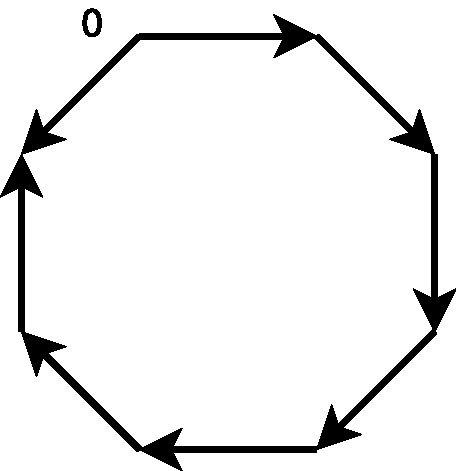
\includegraphics[width=0.3\textwidth]{first.pdf}
  }
  \subfloat[Odd reversed]{
    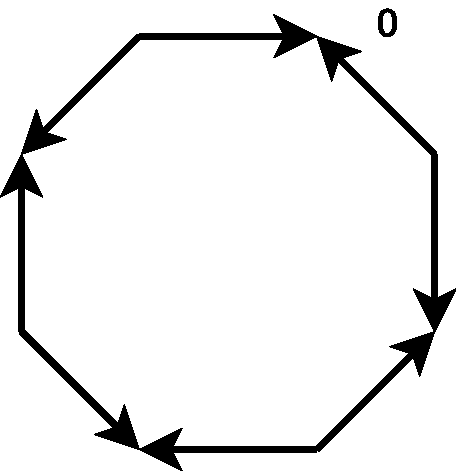
\includegraphics[width=0.3\textwidth]{odd.pdf}
  }
  \caption{Resource dependency graph when first/odd reverse resources
  acquisition order}
  \label{fig:builders}.
\end{figure}


\begin{table}[h!]
  \small
  \framebox{
    \begin{tabular}{ c | c | c c c c | c}
      cooperative & reversed & total time (s) & pause \% & wait \% & work \% & index of dispersion \\
      \hline
      yield & first & 2033.225 & 0.010 & 93.880 & 6.111 & 5282.495 (and growing) \\
      no yield & first & 2017.563 & 0.008 & 93.707 & 6.286 & 5151.709 (and growing) \\
      yield & odd & 2008.691 & 0.046 & 62.209 & 37.745 & 24.072 \\
      no yield & odd & 2001.546 & 0.032 & 63.907 & 36.061 & 26.071 \\
    \end{tabular}
  }
  \caption{Pause, waiting, working times for 20 builders.}
  \label{tbl:builders}
\end{table}

\newpage
\section{Samaritan}

\begin{figure}[h!]
  \small
  \begin{minipage}{0.5\linewidth}
    \begin{Verbatim}[frame=single]
Samaritan
---------
repeat
  synchronize (samaritan)
    picks 2 resources at random
    makes the resources available
    notifies everybody on samaritan
    waits on samaritan

    \end{Verbatim}
  \end{minipage}
  \begin{minipage}{0.5\linewidth}
    \begin{Verbatim}[frame=single]
Player
---------
repeat
  synchronize (samaritan)
    waits on samaritan
    if all resources available
      consumes resources
      builds something (10ms)
      notifies everybody on samaritan
    \end{Verbatim}
  \end{minipage}
  \caption{Pseudocode for Samaritan and Players}
  \label{fig:samaritan-pseudocode}
\end{figure}

The pseudocode for \emph{Samaritan} and \emph{Player} is listed in figure
\ref{fig:samaritan-pseudocode}. There is only one \emph{Samaritan} used
as a monitor by everybody and three Players.

First thing to note is that only one of the four participants can be
active at any given time because of the critical sections guarded by
\texttt{samaritan}. The first participant to act is the Samaritan, the others
wait for his notification. The Samaritan picks two different resources and
makes them available guaranteeing that exactly one Player will be able to
build. Then Samaritan notifies everybody that resources are available and
waits for them to be consumed.

Next, Players wake up one by one in an arbitrary order. If Player wakes and
he does not have all resources he will go back to into waiting state.  If,
however, waked Player has the resources it consumes them. Consequently no other
Player can act until the Samaritan spawns new resources. After the current
Player finishes its actions he notifies everybody including the Samaritan.
If another Player wakes before the Samaritan he will do nothing because he
does not have resources.

Eventually the Samaritan is woken up and the process repeats. It is possible
that now some Players are notified, while others are not. However, it is
irrelevant because Samaritan will notify all Players after it generates
resources.

The algorithm does not deadlock because after a Player consumes the resources
generated by the Samaritan he will wake the Samaritan restarting the
process. At most one set of resources will be available at any
given time because the Samaritan generates resources for exactly one Player
and he is waken again \emph{only} after these resources have been consumed.

No player will starve because every round the Player that will have all the
resources is picked uniformly at random.

\end{document}
